\documentclass[review]{elsarticle}

\usepackage{amsmath}
\usepackage{booktabs}
\usepackage[makeroom]{cancel}
\usepackage[section]{placeins}
\usepackage{subcaption}
\usepackage{tabularx}
\usepackage{nicefrac}
\usepackage[usenames]{xcolor}
\usepackage{lineno,hyperref}
\modulolinenumbers[5]

\journal{Finite Elements in Analysis and Design}

%%%%%%%%%%%%%%%%%%%%%%%
%% Elsevier bibliography styles
%%%%%%%%%%%%%%%%%%%%%%%
%% To change the style, put a % in front of the second line of the current style and
%% remove the % from the second line of the style you would like to use.
%%%%%%%%%%%%%%%%%%%%%%%

%% Numbered
%\bibliographystyle{model1-num-names}

%% Numbered without titles
%\bibliographystyle{model1a-num-names}

%% Harvard
%\bibliographystyle{model2-names.bst}\biboptions{authoryear}

%% Vancouver numbered
%\usepackage{numcompress}\bibliographystyle{model3-num-names}

%% Vancouver name/year
%\usepackage{numcompress}\bibliographystyle{model4-names}\biboptions{authoryear}

%% APA style
%\bibliographystyle{model5-names}\biboptions{authoryear}

%% AMA style
%\usepackage{numcompress}\bibliographystyle{model6-num-names}

%% `Elsevier LaTeX' style
\bibliographystyle{elsarticle-num}
%%%%%%%%%%%%%%%%%%%%%%%

\begin{document}

\begin{frontmatter}

\title{Eigenbasis of the discrete Energy Release Rate and mode partition for the Virtual Crack Closure Technique (VCCT) in the context of 2D the Finite Element Method (FEM)}
%\tnotetext[mytitlenote]{Fully documented templates are available in the elsarticle package on \href{http://www.ctan.org/tex-archive/macros/latex/contrib/elsarticle}{CTAN}.}

%% Group authors per affiliation:
%\author{Luca Di Stasio\fnref{myfootnote}}
%\address{Radarweg 29, Amsterdam}
%\fntext[myfootnote]{Since 1880.}

%% or include affiliations in footnotes:
\author[lulea]{Luca Di Stasio}
%\author[lulea]{Janis Varna}
%\author[nancy]{Zoubir Ayadi}
%\ead[url]{www.elsevier.com}

%\author[mysecondaryaddress]{Global Customer Service\corref{mycorrespondingauthor}}
%\cortext[mycorrespondingauthor]{Corresponding author}
%\ead{support@elsevier.com}

\address[lulea]{Lule\aa\ University of Technology, University Campus, SE-97187 Lule\aa, Sweden}
%\address[nancy]{Universit\'e de Lorraine, EEIGM, IJL, 6 Rue Bastien Lepage, F-54010 Nancy, France}

\begin{abstract}
\noindent

\end{abstract}

\begin{keyword}
Fiber/matrix interface crack\sep Bi-material interface arc crack\sep Linear Elastic Fracture Mechanics (LEFM)\sep Virtual Crack Closure Technique (VCCT) \sep Mode separation\sep Eigenbasis
\end{keyword}

\end{frontmatter}

\linenumbers

\section{Introduction}\label{sec:intro}



\section{FEM formulation of the fiber-matrix interface crack problem}\label{sec:femmodel}



\section{Vectorial formulation of the Virtual Crack Closure Technique (VCCT)}
 
In order to express the VCCT formulation of the ERR in terms of FEM variables, we need to introduce a few rotation matrices in order to represent the discretized representation (FE mesh) of a crack along a circular interface. The position of the crack tip is characterized by the angular size of the crack (see Sec.~\ref{sec:femmodel} and Fig.~\ref{fig:modelschem} for reference) and the rotation corresponding to the crack tip reference frame is represented by the matrix $\underline{\underline{R}}_{\Delta\theta}$ defined as

\begin{equation}\label{eq:Rmatrix}
\underline{\underline{R}}_{\Delta\theta}=\begin{bmatrix}
\cos\left(\Delta\theta\right) & \sin\left(\Delta\theta\right) \\
-\sin\left(\Delta\theta\right) & \cos\left(\Delta\theta\right)
\end{bmatrix}.
\end{equation}

Nodes belonging to the elements sharing the crack tip are involved in the VCCT estimation of the ERR and it is assumed that, given a sufficiently fine discretization, they are aligned with the crack propagation direction defined at the crack tip. However, irrespectively of how small the elements in the crack tip neighborhood are, a misalignment always exists with respect to the assumed crack propagation direction (in the crack tip reference frame). This is measured by the matrices $\underline{\underline{P}}_{\delta}\left(p\right)$, defined as

\begin{equation}\label{eq:Pmatrix}
\underline{\underline{P}}_{\delta}\left(p\right)=\begin{bmatrix}
\cos\left(\left(1+\frac{1-p}{m}\right)\delta\right) & \sin\left(\left(1+\frac{1-p}{m}\right)\delta\right) \\
-\sin\left(\left(1+\frac{1-p}{m}\right)\delta\right) & \cos\left(\left(1+\frac{1-p}{m}\right)\delta\right)
\end{bmatrix}
\end{equation}

 and $\underline{\underline{Q}}_{\delta}\left(q\right)$, equal to 

\begin{equation}\label{eq:Qmatrix}
\underline{\underline{Q}}_{\delta}\left(q\right)=\begin{bmatrix}
\cos\left(\frac{q-1}{m}\delta\right) & \sin\left(\frac{q-1}{m}\delta\right) \\
-\sin\left(\frac{q-1}{m}\delta\right) & \cos\left(\frac{q-1}{m}\delta\right)
\end{bmatrix},
\end{equation}

respectively for the free and bonded nodes involved in the VCCT estimation. In Eqs.~\ref{eq:Pmatrix} and~\ref{eq:Qmatrix}, $\delta$ is the angular size of an element in the crack tip neighborhood (see Sec.~\ref{sec:femmodel} and Fig.~\ref{fig:modelschem}), $m$ is the order of the element shape functions and $p,q$ are indices referring to the nodes belonging respectively to free and bonded elements sharing the crack tip. Introducing the permutation matrix


\begin{equation}
\underline{\underline{P}}_{\pi}=\begin{bmatrix}
0 & 1\\
-1& 0
\end{bmatrix},
\end{equation}

it is possible to express the derivatives of rotation matrices $\underline{\underline{R}}_{\Delta\theta}$, $\underline{\underline{P}}_{\delta}$ and $\underline{\underline{Q}}_{\delta}$ with respect to their argument:

\begin{equation}\label{eq:rotmatdev}
\frac{\partial \underline{\underline{R}}_{\Delta\theta}}{\partial \Delta\theta}=\underline{\underline{D}}\cdot\underline{\underline{R}}_{\Delta\theta},\quad\frac{\partial \underline{\underline{P}}_{\delta}}{\partial \delta}=\left(1+\frac{1-p}{m}\right)\underline{\underline{D}}\cdot\underline{\underline{P}}_{\delta},\quad\frac{\partial \underline{\underline{Q}}_{\delta}}{\partial \delta}=\frac{q-1}{m}\underline{\underline{D}}\cdot\underline{\underline{Q}}_{\delta}.
\end{equation}

By means of Eqs.~\ref{eq:Pmatrix} and~\ref{eq:Qmatrix}, we can express the crack tip forces $
\underline{F}_{xy}=\begin{bmatrix}
F_{x} \\
F_{y}
\end{bmatrix}$ and crack displacements  $
\underline{u}_{xy}=\begin{bmatrix}
u_{x} \\
u_{y}
\end{bmatrix}$ in the crack tip reference frame (where the tangential direction $\theta$ correspond to the direction of crack propagation) while taking into account the misalignment to the finite  discretization as 

\begin{equation}\label{eq:FUrot}
\underline{F}_{r\theta}=\underline{\underline{Q}}_{\delta}\underline{\underline{R}}_{\Delta\theta}\underline{F}_{xy}\qquad\underline{u}_{r\theta}=\underline{\underline{P}}_{\delta}\underline{\underline{R}}_{\Delta\theta}\underline{u}_{xy}
\end{equation}

where $\underline{F}_{r\theta}=\begin{bmatrix}
F_{r} \\
F_{\theta}
\end{bmatrix}$ and $\underline{u}_{r\theta}=\begin{bmatrix}
u_{r} \\
u_{\theta}
\end{bmatrix}$.

The crack tip forces can be expressed as a function of the crack opening displacement as 

\begin{equation}\label{eq:ctforce1}
\underline{F}_{xy}=\underline{\underline{K}}_{xy}\underline{u}_{xy}+\underline{\widetilde{F}}_{xy},
\end{equation}
 
where $\underline{\underline{K}}_{xy}$ is in general a full matrix of the form $\underline{\underline{K}}_{xy}=\begin{bmatrix}
K_{xx}  K_{xy}\\
K_{yx}  K_{yy}
\end{bmatrix}$ and $\underline{\widetilde{F}}_{xy}$ represents the effect of the rest of the FE solution through the remaining nodes of the elements attached to the crack tip. As such, the term $\underline{\widetilde{F}}_{xy}$ can be expressed as a linear combination of the solution vector $\underline{u}_{N}$ of nodal displacements of the form $\underline{\underline{\widetilde{K}}}_{N}\underline{u}_{N}$. Equation~\ref{eq:ctforce1} thus become

\begin{equation}\label{eq:ctforce2}
\underline{F}_{xy}=\underline{\underline{K}}_{xy}\underline{u}_{xy}+\underline{\underline{\widetilde{K}}}_{N}\underline{u}_{N}.
\end{equation}

An exemplifying derivation of the relationships expressed in Equations~\ref{eq:ctforce1} and~\ref{eq:ctforce2} can be found in \ref{app:ctforcesexample}. It is worthwhile to observe that another author~\cite{Valvo2011} proposed a relationship of the form $\underline{F}_{xy}=\underline{\underline{K}}_{xy}\underline{u}_{xy}$. However, in~\cite{Valvo2011}, this relationship is assumed \emph{a priori} and manipulated to propose a revised version of the VCCT, based on the assumption that the matrix $\underline{\underline{K}}_{xy}$ should be diagonal to provide physically-consistent fracture mode partitioning. On the other hand, in the present work we derive the relationships of Eqs.~\ref{eq:ctforce1} and~\ref{eq:ctforce2} from the formulation of the Finite Element Method. According to our derivation, it seems correct that the matrix $\underline{\underline{K}}_{xy}$ should not in general be diagonal in order to take into account Poisson's effect. In fact, a positive crack opening displacement would cause a transverse displacement in the neighborhood of the crack tip. Given that material properties are different on the two sides of a bi-material interface, a net shear would be applied to the crack tip which would correspond to a net contribution to the crack tip force related to crack shear displacement. The analytical derivations presented in \ref{app:ctforcesexample} confirm these physical considerations.\\
Based upon the work of Raju~\cite{Raju1987}, we introduce the matrix $\underline{\underline{T}}_{pq}$ to represent the weights needed in the VCCT to account for the use of singular elements. As already done previously, indices $p$ and $q$ refer to nodes placed respectively on the free (crack face) and bonded side of the crack tip. Nodes are enumerated so that the crack tip has always index $1$, i.e. the higher the index the further the node is from the crack tip. Matrix $\underline{\underline{T}}_{pq}$ has always a size of $d\times d$, where $d=2$ for a $2D$ problem and $d=3$ for a $3D$ problem. An element $\underline{\underline{T}}_{pq}\left(i,j\right)$ with $i,j=1,\dots,d$ represents the weight to be assigned to the product of component $i$ of the displacement extracted at node $p$ with component $j$ of the force extracted at node $q$. The expression of $\underline{\underline{T}}_{pq}$ for quadrilateral elements with or without singularity is reported in \ref{app:Tpq}. Notice that, given $m$ is the order of the element shape functions, the element side has $m+1$ nodes and this represents the upper limit of indices $p$ and $q$.\\
By using matrix $\underline{\underline{T}}_{pq}$, it is possible to express the total ERR $G$ evaluated with the VCCT as

\begin{equation}\label{eq:gtot}
G_{TOT} = \frac{1}{2R_{f}\delta}\sum_{p=1}^{m+1}\sum_{q=1}^{m+1}Tr\left(\underline{u}_{r\theta,p}^{T}\underline{\underline{T}}_{pq}^{T}\underline{F}_{r\theta,q}\right).
\end{equation}

Introducing the vector $\underline{G}=\begin{bmatrix}
G_{I} \\
G_{II}
\end{bmatrix}$ of fracture mode ERRs, Mode I and Mode II ERR evaluated with the VCCT can be expressed as 

\begin{equation}\label{eq:g}
\underline{G} =\frac{1}{2R_{f}\delta}\sum_{p=1}^{m+1}\sum_{q=1}^{m+1}Diag\left(\underline{F}_{r\theta,q}\underline{u}_{r\theta,p}^{T}\underline{\underline{T}}_{pq}^{T}\right),
\end{equation}

where $Diag\left(\right)$ is the function that extracts the main diagonal of the input matrix as a column vector. Substituting Equations~\ref{eq:FUrot} and~\ref{eq:ctforce2} in Equations~\ref{eq:gtot} and~\ref{eq:g}, we can express the Mode I, Mode II and total Energy Release Rate as a function of the crack displacements and the FE solution (more details in \ref{app:ctforcesexample}) as 

\begin{equation}\label{eq:gtotlong}
\begin{split}
G_{TOT} =&\frac{1}{2R_{f}\delta}\sum_{p=1}^{m+1}\sum_{q=1}^{m+1}Tr\left(\underline{\underline{Q}}_{\delta}\underline{\underline{R}}_{\Delta\theta}\underline{\underline{K}}_{xy,q}\underline{u}_{xy,q}\underline{u}_{xy,p}^{T}\underline{\underline{R}}_{\Delta\theta}^{T}\underline{\underline{P}}_{\delta}^{T}\underline{\underline{T}}_{pq}^{T}\right)+\\&+\frac{1}{2R_{f}\delta}\sum_{p=1}^{m+1}\sum_{q=1}^{m+1}Tr\left(\underline{\underline{Q}}_{\delta}\underline{\underline{R}}_{\Delta\theta}\underline{\widetilde{F}}_{xy,q}\underline{u}_{xy,p}^{T}\underline{\underline{R}}_{\Delta\theta}^{T}\underline{\underline{P}}_{\delta}^{T}\underline{\underline{T}}_{pq}^{T}\right)
\end{split}
\end{equation}

and

\begin{equation}
\begin{split}
\underline{G}=\begin{bmatrix}
G_{I} \\
G_{II}
\end{bmatrix}=&\frac{1}{2R_{f}\delta}\sum_{p=1}^{m+1}\sum_{q=1}^{m+1}Diag\left(\underline{\underline{Q}}_{\delta}\underline{\underline{R}}_{\Delta\theta}\underline{\underline{K}}_{xy,q}\underline{u}_{xy,q}\underline{u}_{xy,p}^{T}\underline{\underline{R}}_{\Delta\theta}^{T}\underline{\underline{P}}_{\delta}^{T}\underline{\underline{T}}_{pq}^{T}\right)+\\
&+\frac{1}{2R_{f}\delta}\sum_{p=1}^{m+1}\sum_{q=1}^{m+1}Diag\left(\underline{\underline{Q}}_{\delta}\underline{\underline{R}}_{\Delta\theta}\underline{\underline{\widetilde{K}}}_{N,q}\underline{u}_{N}\underline{u}_{xy,p}^{T}\underline{\underline{R}}_{\Delta\theta}^{T}\underline{\underline{P}}_{\delta}^{T}\underline{\underline{T}}_{pq}^{T}\right)
\end{split}
\end{equation}

\begin{equation}
\underline{\underline{A}}=\underline{\underline{Q}}_{\delta}\underline{\underline{R}}_{\Delta\theta}\left(\underline{\underline{K}}_{xy,q}\underline{u}_{xy,q}+\underline{\underline{\widetilde{K}}}_{N,q}\underline{u}_{N}\right)\underline{u}_{xy,p}^{T}\underline{\underline{R}}_{\Delta\theta}^{T}\underline{\underline{P}}_{\delta}^{T}\underline{\underline{T}}_{pq}^{T}
\end{equation}

\begin{equation}
\det\left(\underline{\underline{A}}-\lambda\underline{\underline{I}}\right)=\det\left(\underline{\underline{Q}}_{\delta}\underline{\underline{R}}_{\Delta\theta}\left(\underline{\underline{K}}_{xy,q}\underline{u}_{xy,q}+\underline{\underline{\widetilde{K}}}_{N,q}\underline{u}_{N}\right)\underline{u}_{xy,p}^{T}\underline{\underline{R}}_{\Delta\theta}^{T}\underline{\underline{P}}_{\delta}^{T}\underline{\underline{T}}_{pq}^{T}-\lambda\underline{\underline{I}}\right)=0
\end{equation}

\begin{equation}
\det\left(\underline{\underline{A}}-\lambda\underline{\underline{I}}\right)=\det\left(\begin{bmatrix}
A_{11}-\lambda&A_{12} \\
A_{21}&A_{22}-\lambda
\end{bmatrix}\right)=0
\end{equation}

\begin{equation}
\lambda^{2}-\left(A_{11}+A_{22}\right)\lambda+\left(A_{11}A_{22}-A_{12}A_{21}\right)=0
\end{equation}

\begin{equation}
\lambda_{1,2}=\frac{1}{2}\left(-\left(A_{11}+A_{22}\right)\pm\sqrt{\left(A_{11}+A_{22}\right)^{2}-4\left(A_{11}A_{22}-A_{12}A_{21}\right)}\right)
\end{equation}

\section{Conclusions \& Outlook}



\FloatBarrier

\section*{Acknowledgements}



\bibliography{refs}

\appendix
\section{Derivation of the relationship between crack tip forces and displacements for first order quadrilateral elements}\label{app:ctforcesexample}

\subsection{Foundational relations}

In the isoparametric formulation of the Finite Element Method, the element Jacobian $J$ and its inverse $J^{-1}$ can be expressed in general as 

\begin{equation}
\underline{\underline{J}}=\begin{bmatrix}
\underline{e}_{\xi}|\underline{e}_{\eta}
\end{bmatrix}=\begin{bmatrix}
\frac{\partial x}{\partial\xi}&\frac{\partial x}{\partial\eta}\\\frac{\partial y}{\partial\xi}&\frac{\partial y}{\partial\eta}
\end{bmatrix}\qquad\underline{\underline{J}}^{-1}=\begin{bmatrix}
\underline{e}^{x}|\underline{e}^{y}
\end{bmatrix}=\begin{bmatrix}
\frac{\partial \xi}{\partial x}&\frac{\partial \xi}{\partial y}\\\frac{\partial \eta}{\partial x}&\frac{\partial \eta}{\partial y}
\end{bmatrix}
\end{equation}

where $\left\{e_{\xi}, e_{\eta}\right\}$ and $\left\{e^{x}, e^{y}\right\}$ are respectively the covariant and contravariant basis vectors of the mapping between global $\left\{x, y\right\}$ and local element $\left\{\xi, \eta\right\}$ coordinates:

\begin{equation}
\underline{e}_{\xi}=\begin{bmatrix}
\frac{\partial x}{\partial\xi}\\\frac{\partial y}{\partial\xi}
\end{bmatrix}\quad\underline{e}_{\eta}=\begin{bmatrix}
\frac{\partial x}{\partial\eta}\\\frac{\partial y}{\partial\eta}
\end{bmatrix},
\end{equation}

\begin{equation}
\underline{e}_{x}=\begin{bmatrix}
\frac{\partial \xi}{\partial x}\\\frac{\partial \eta}{\partial x}
\end{bmatrix}\quad\underline{e}_{y}=\begin{bmatrix}
\frac{\partial \xi}{\partial y}\\\frac{\partial \eta}{\partial y}
\end{bmatrix}.
\end{equation}

Denoting by $d$ the number of geometrical dimensions of the problem ($d=2$ in the present work) and by $\underline{p}$ the $d\times 1$ position vector in global coordinates, we can formally introduce the $3\left(d-1\right)\times d$ matrix operator of partial differentiation $\underline{\underline{\widetilde{B}}}$ such that

\begin{equation}\label{eq:introB}
\underline{\varepsilon}\left(\underline{p}\right)=\underline{\underline{\widetilde{B}}}\cdot\underline{u}\left(\underline{p}\right),
\end{equation}

where $\underline{u}$ and $\underline{\varepsilon}$ are respectively the $d\times 1$ displacement vector and the $3\left(d-1\right)\times 1$ strain vector in Voigt notation. Denoting by $n$ the number of nodes of a generic element ($n=s\times m$ where $s$ represents the number of sides of the element and $m$ the order of the shape functions), we can furthermore introduce the $d\times d\cdot n$ matrix \underline{\underline{N}} of shape functions such that

\begin{equation}\label{eq:introN}
\underline{u}=\underline{\underline{N}}\cdot\underline{u}_{N},
\end{equation}

where $\underline{u}_{N}$ is the $d\cdot n\times 1$ vector of element nodal variables. Having introduced $\underline{\underline{\widetilde{B}}}$ and $\underline{\underline{N}}$ in Equations~\ref{eq:introB} and~\ref{eq:introN} respectively, it is possible to define the $3\left(d-1\right)\times d\cdot n$ matrix $\underline{\underline{B}}$ of derivatives (with respect to global coordinates) of shape functions as

\begin{equation}
\underline{\underline{B}}=\underline{\underline{\widetilde{B}}}\cdot\underline{\underline{N}}.
\end{equation}

We introduce the linear elastic material behavior in the form of the $3\left(d-1\right)\times 3\left(d-1\right)$ rigidity matrix $\underline{\underline{D}}$ such that

\begin{equation}
\underline{\sigma}=\underline{\underline{D}}\cdot\underline{\varepsilon},
\end{equation}

where $\underline{\sigma}$ the $3\left(d-1\right)\times 1$ stress vector in Voigt notation. It is finally possible to define the $n\times n$ element stiffness matrix $\underline{\underline{k_{e}}}$ as 

\begin{equation}\label{eq:elestiff}
\underline{\underline{k_{e}}}=\int_{V_{e}\left(x,y\right)}\left(\underline{\underline{B}}^{T}\underline{\underline{D}}\cdot\underline{\underline{B}}\right)dV_{e}\left(x,\dots,y\right)=\int_{V_{e}\left(\xi,\eta\right)}\left(\underline{\underline{B}}^{T}\underline{\underline{D}}\cdot\underline{\underline{B}}\right)\sqrt{g}dV_{e}\left(\xi,\dots,\eta\right),
\end{equation}

where $g=det\left(\underline{\underline{J}}^{T}\underline{\underline{J}}\right)$ and $V_{e}$ is the element volume. Given that isoparametric elements are always defined between $-1$ and $1$ in each dimension, Equation~\ref{eq:elestiff} can simplified to

\begin{equation}
\underline{\underline{k_{e}}}=\int_{-1}^{1}\dots\int_{-1}^{1}\left(\underline{\underline{B}}^{T}\underline{\underline{D}}\cdot\underline{\underline{B}}\right)\sqrt{g}d\xi,\dots, d\eta,
\end{equation}

which is amenable to numerical integration by means of a Gaussian quadrature of the form

\begin{equation}\label{eq:elstiffnum}
\underline{\underline{k_{e}}}\approx \sum_{i=1}^{N}\dots\sum_{j=1}^{N}w_{i}\dots w_{j}\left(\underline{\underline{B}}^{T}\left(\xi_{i}, \dots,\eta_{j}\right)\cdot\underline{\underline{D}}\cdot\underline{\underline{B}}\left(\xi_{i}, \dots,\eta_{j}\right)\sqrt{g}\right),
\end{equation}

where $\left(\xi_{i}, \dots,\eta_{j}\right)$ are the coordinates of the $N$ Gaussian quadrature points. The element stiffness matrix as evaluated in Eq.~\ref{eq:elstiffnum} is in general a full symmetric (in the case of linear elasticity) matrix of the form

\begin{equation}\label{eq:elstiffmatrix}
k_{e}=\begin{bmatrix}
k_{e|11}&k_{e|12}&k_{e|13}&k_{e|14}&k_{e|15}&k_{e|16}&k_{e|17}&k_{e|18}\\
k_{e|12}&k_{e|22}&k_{e|23}&k_{e|24}&k_{e|25}&k_{e|26}&k_{e|27}&k_{e|28}\\
k_{e|13}&k_{e|23}&k_{e|33}&k_{e|34}&k_{e|35}&k_{e|36}&k_{e|37}&k_{e|38}\\
k_{e|14}&k_{e|24}&k_{e|34}&k_{e|44}&k_{e|45}&k_{e|46}&k_{e|47}&k_{e|48}\\
k_{e|15}&k_{e|25}&k_{e|35}&k_{e|45}&k_{e|55}&k_{e|56}&k_{e|57}&k_{e|58}\\
k_{e|16}&k_{e|26}&k_{e|36}&k_{e|46}&k_{e|56}&k_{e|66}&k_{e|67}&k_{e|68}\\
k_{e|17}&k_{e|27}&k_{e|37}&k_{e|47}&k_{e|57}&k_{e|67}&k_{e|77}&k_{e|78}\\
k_{e|18}&k_{e|28}&k_{e|38}&k_{e|48}&k_{e|58}&k_{e|68}&k_{e|78}&k_{e|88}\\
\end{bmatrix}.
\end{equation}

\subsection{Calculation of displacements and reaction forces}

With reference to Fig.~\ref{fig:vcctlinear}, we define:

\begin{description}
\item[$u_{x,M}$, $u_{x,F}$] the $x$-displacement of the nodes belonging to the free side of the first element belonging to the crack, respectively on the matrix (bulk) and fiber (inclusion) side;
\item[$u_{y,M}$, $u_{y,F}$] the $y$-displacement of the nodes belonging to the free side of the first element belonging to the crack, respectively on the matrix (bulk) and fiber (inclusion) side;
\item[$u_{r,M}$, $u_{r,F}$] the $x$-displacement of the nodes belonging to the free side of the first element belonging to the crack, respectively on the matrix (bulk) and fiber (inclusion) side;
\item[$u_{\theta,M}$, $u_{\theta,F}$] the $y$-displacement of the nodes belonging to the free side of the first element belonging to the crack, respectively on the matrix (bulk) and fiber (inclusion) side;
\item[$F_{x,CT}$, $F_{y,CT}$] respectively the $x$- and $y$-component of the reaction force at the crack tip;
\item[$F_{r,CT}$, $F_{\theta,CT}$] respectively the $r$- and $\theta$-component of the reaction force at the crack tip.
\end{description}

The $x-y$ reference frame is the global reference frame, while the $r-\theta$ reference frame is such that the $\theta$ direction coincides with the crack propagation direction at the crack tip and $r$ the in-plane normal to the propagation direction. For an arc-crack as the present one, the $r$-direction coincides with the radial direction of the inclusion.

%\begin{figure}[!h]
%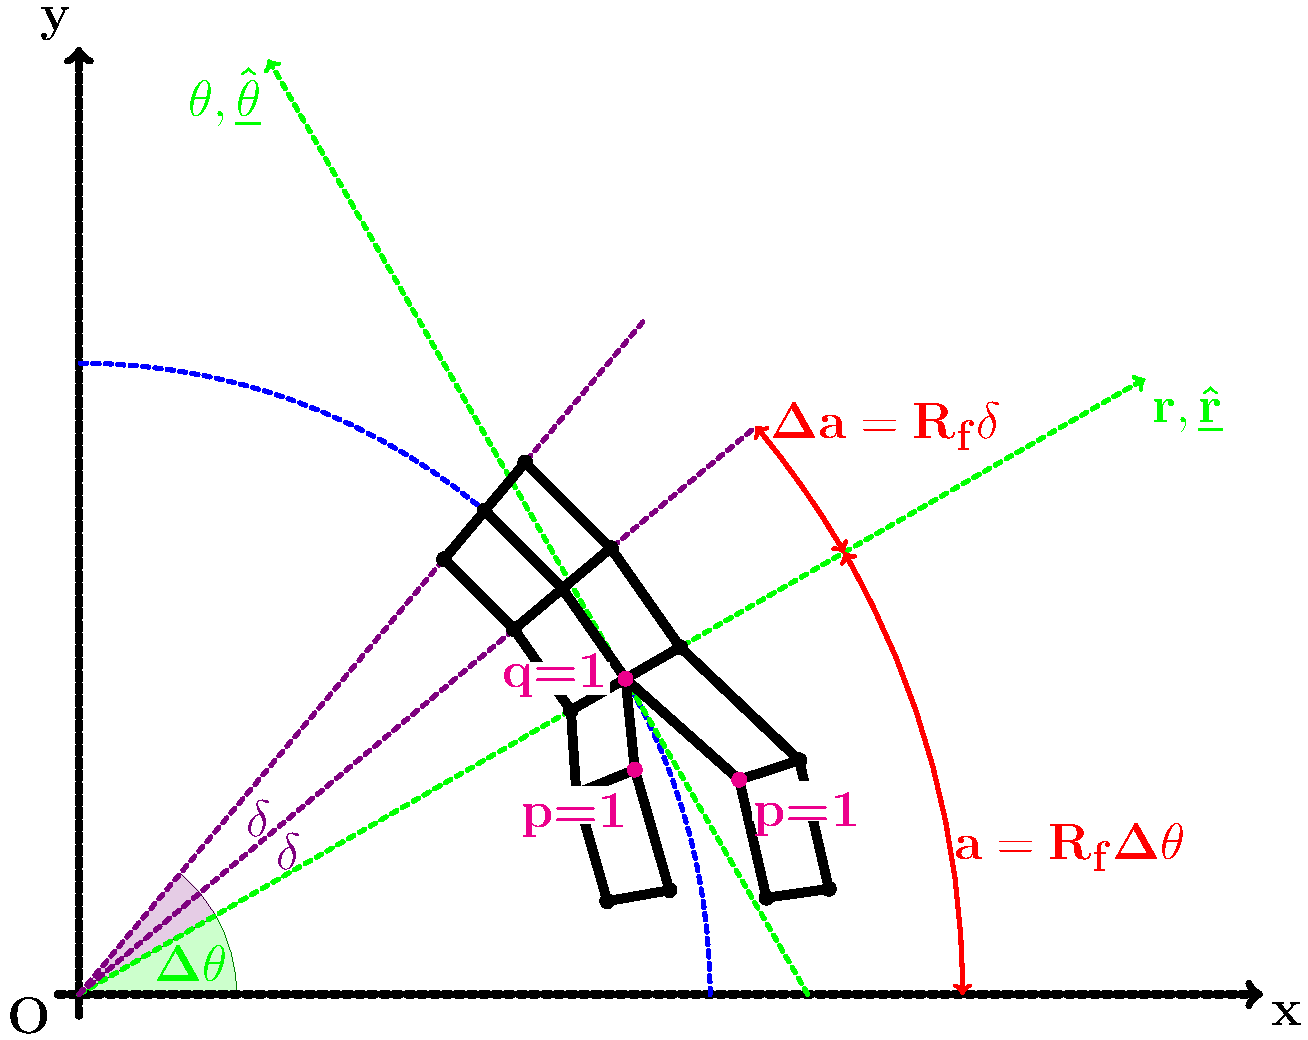
\includegraphics[width=\textwidth]{VCCT-linear.pdf}
%\caption{Schematic representation of the discretized crack tip geometry for  $1^{st}$ order quadrilateral elements.}\label{fig:vcctlinear}
%\end{figure}

The crack opening displacement $u_{r}$ and the crack shear displacement $u_{\theta}$ at the crack tip can thus be written as

\begin{equation}
u_{r}=\cos\left(\Delta\theta\right) u_{x}+\sin\left(\Delta\theta\right) u_{y}\qquad u_{\theta}=-\sin\left(\Delta\theta\right) u_{x}+\cos\left(\Delta\theta\right) u_{y},
\end{equation}

where $u_{x}$ and $u_{y}$ are defined as

\begin{equation}\label{eq:uxuy}
u_{x}=u_{x,M}-u_{x,F}\qquad u_{y}=u_{y,M}-u_{y,F}
\end{equation}

and $2\Delta\theta$ is total angular size of the debond. The corresponding forces at the crack tip are

\begin{equation}
F_{r}=\cos\left(\Delta\theta\right) F_{x,CT}+\sin\left(\Delta\theta\right) F_{y,CT}\qquad F_{\theta}=-\sin\left(\Delta\theta\right) F_{x,CT}+\cos\left(\Delta\theta\right) F_{y,CT}.
\end{equation}

At the crack tip, the FE mesh possesses two coincident points, labeled $FCT$ and $MCT$. Continuity of the displacements at the crack tip must be ensured. Furthermore, in order to measure the force at the crack tip, a fully-constraint dummy node needs to be created and formally linked to the two nodes at the crack tip by the conditions 

\begin{equation}
\begin{cases}
&u_{x,FCT}-u_{x,MCT}-u_{x,DUMMY}=0\\
&u_{y,FCT}-u_{y,MCT}-u_{y,DUMMY}=0\\[10pt]
&u_{x,DUMMY}=0\\
&u_{y,DUMMY}=0\\
\end{cases},
\end{equation}

which can be simplified to

\begin{equation}
\begin{cases}
&u_{x,FCT}=u_{x,MCT}\\
&u_{y,FCT}=u_{y,MCT}\\[10pt]
&R_{x,DUMMY}=R_{x,FCT}=-R_{x,MCT}=F_{x,CT}\\
&R_{y,DUMMY}=R_{y,FCT}=-R_{y,MCT}=F_{y,CT}\\
\end{cases}.
\end{equation}

Making use of Eq.~\ref{eq:elstiffmatrix}, four equations can be written in the four displacement $u_{x,FCT}$, $u_{x,MCT}$, $u_{y,FCT}$ and $u_{y,MCT}$:

\begin{equation}\label{eq:syseqs01}
\begin{cases}
&\left(k_{e,M|11}+k_{e,M|33}\right)u_{x,MCT}+\left(k_{e,M|12}+k_{e,M|34}\right)u_{y,MCT}+\\&+k_{e,M|13}u_{x,M}+k_{e,M|14}u_{y,M}+\left(k_{M|17}+k_{M|35}\right)u_{N,MC|7}+\left(k_{M|18}+k_{M|36}\right)u_{N,MC|8}+\\&+\sum_{i=5}^{6}k_{M|1i}u_{N,MC|i}+\sum_{i=7}^{8}k_{M|3i}u_{N,MB|i}+k_{M|31}u_{x,NCOI}+k_{M|32}u_{y,NCOI}=0\\[10pt]
&\left(k_{e,M|21}+k_{e,M|43}\right)u_{x,MCT}+\left(k_{e,M|22}+k_{e,M|44}\right)u_{y,MCT}+\\&+k_{e,M|23}u_{x,M}+k_{e,M|24}u_{y,M}+\left(k_{M|27}+k_{M|45}\right)u_{N,MC|7}+\left(k_{M|28}+k_{M|46}\right)u_{N,MC|8}+\\&+\sum_{i=5}^{6}k_{M|2i}u_{N,MC|i}+\sum_{i=7}^{8}k_{M|4i}u_{N,MB|i}+k_{M|41}u_{x,NCOI}+k_{M|42}u_{y,NCOI}=0\\[10pt]
&\left(k_{e,F|77}+k_{e,F|55}\right)u_{x,FCT}+\left(k_{e,F|78}+k_{e,F|56}\right)u_{y,FCT}+\\&+k_{e,F|75}u_{x,F}+k_{e,F|76}u_{y,F}+\left(k_{F|71}+k_{F|53}\right)u_{N,FC|1}+\left(k_{F|72}+k_{F|54}\right)u_{N,FC|2}+\\&+\sum_{i=2}^{3}k_{F|7i}u_{N,FC|i}+\sum_{i=1}^{2}k_{F|5i}u_{N,FB|i}+k_{F|57}u_{x,NCOI}+k_{F|58}u_{y,NCOI}=0\\[10pt]
&\left(k_{e,F|87}+k_{e,F|65}\right)u_{x,FCT}+\left(k_{e,F|88}+k_{e,F|66}\right)u_{y,FCT}+\\&+k_{e,F|85}u_{x,F}+k_{e,F|86}u_{y,F}+\left(k_{F|81}+k_{F|63}\right)u_{N,FC|1}+\left(k_{F|82}+k_{F|64}\right)u_{N,FC|2}+\\&+\sum_{i=2}^{3}k_{F|8i}u_{N,FC|i}+\sum_{i=1}^{2}k_{F|6i}u_{N,FB|i}+k_{F|67}u_{x,NCOI}+k_{F|68}u_{y,NCOI}=0\\[10pt]
\end{cases}.
\end{equation}

Solving for $u_{y,FCT}$ and $u_{y,MCT}$ the third and fourth relations in Eq.~\ref{eq:syseqs01} and substituting in the first two expressions of Eq.~\ref{eq:syseqs01}, we get

\begin{equation}\label{eq:syseqs02}
\footnotesize
\begin{cases}
&\left(k_{e,M|11}+k_{e,M|33}+k_{e,F|77}+k_{e,F|55}\right)u_{x,MCT}+\left(k_{e,M|12}+k_{e,M|34}+k_{e,F|78}+k_{e,F|56}\right)u_{y,MCT}+\\&+k_{e,M|13}u_{x,M}+k_{e,M|14}u_{y,M}+k_{e,F|75}u_{x,F}+k_{e,F|76}u_{y,F}+\\&+\left(k_{M|31}+k_{F|57}\right)u_{x,NCOI}+\left(k_{M|32}+k_{F|58}\right)u_{y,NCOI}+\\&+\left(k_{M|17}+k_{M|35}\right)u_{N,MC|7}+\left(k_{M|18}+k_{M|36}\right)u_{N,MC|8}+\left(k_{F|71}+k_{F|53}\right)u_{N,FC|1}+\left(k_{F|72}+k_{F|54}\right)u_{N,FC|2}+\\&+\sum_{i=5}^{6}k_{M|1i}u_{N,MC|i}+\sum_{i=7}^{8}k_{M|3i}u_{N,MB|i}+\sum_{i=2}^{3}k_{F|7i}u_{N,FC|i}+\sum_{i=1}^{2}k_{F|5i}u_{N,FB|i}=0\\[10pt]
&\left(k_{e,M|21}+k_{e,M|43}+k_{e,F|87}+k_{e,F|65}\right)u_{x,MCT}+\left(k_{e,M|22}+k_{e,M|44}+k_{e,F|88}+k_{e,F|66}\right)u_{y,MCT}+\\&+k_{e,M|23}u_{x,M}+k_{e,M|24}u_{y,M}+k_{e,F|85}u_{x,F}+k_{e,F|86}u_{y,F}+\\&+\left(k_{M|41}+k_{F|67}\right)u_{x,NCOI}+\left(k_{M|42}+k_{F|68}\right)u_{y,NCOI}+\\&+\left(k_{M|27}+k_{M|45}\right)u_{N,MC|7}+\left(k_{M|28}+k_{M|46}\right)u_{N,MC|8}+\left(k_{F|81}+k_{F|63}\right)u_{N,FC|1}+\left(k_{F|82}+k_{F|64}\right)u_{N,FC|2}+\\&+\sum_{i=2}^{3}k_{F|8i}u_{N,FC|i}+\sum_{i=1}^{2}k_{F|6i}u_{N,FB|i}+\sum_{i=5}^{6}k_{M|2i}u_{N,MC|i}+\sum_{i=7}^{8}k_{M|4i}u_{N,MB|i}=0\\[10pt]
\end{cases}
\end{equation}

%\begin{equation}
%\scriptsize
%\begin{cases}
%&u_{y,MCT}=-\frac{k_{e,M|11}+k_{e,M|33}+k_{e,F|77}+k_{e,F|55}}{k_{e,M|12}+k_{e,M|34}+k_{e,F|78}+k_{e,F|56}}u_{x,MCT}+\\
%&-\frac{k_{e,M|13}u_{x,M}+k_{e,M|14}u_{y,M}+k_{e,F|75}u_{x,F}+k_{e,F|76}u_{y,F}}{k_{e,M|12}+k_{e,M|34}+k_{e,F|78}+k_{e,F|56}}+\\
%&-\frac{\left(k_{M|31}+k_{F|57}\right)u_{x,NCOI}+\left(k_{M|32}+k_{F|58}\right)u_{y,NCOI}}{k_{e,M|12}+k_{e,M|34}+k_{e,F|78}+k_{e,F|56}}+\\
%&-\frac{\left(k_{M|17}+k_{M|35}\right)u_{N,MC|7}+\left(k_{M|18}+k_{M|36}\right)u_{N,MC|8}+\left(k_{F|71}+k_{F|53}\right)u_{N,FC|1}+\left(k_{F|72}+k_{F|54}\right)u_{N,FC|2}}{k_{e,M|12}+k_{e,M|34}+k_{e,F|78}+k_{e,F|56}}+\\
%&-\frac{\sum_{i=5}^{6}k_{M|1i}u_{N,MC|i}+\sum_{i=7}^{8}k_{M|3i}u_{N,MB|i}+\sum_{i=2}^{3}k_{F|7i}u_{N,FC|i}+\sum_{i=1}^{2}k_{F|5i}u_{N,FB|i}}{k_{e,M|12}+k_{e,M|34}+k_{e,F|78}+k_{e,F|56}}\\[10pt]
%
%&\left[\left(k_{e,M|21}+k_{e,M|43}+k_{e,F|87}+k_{e,F|65}\right)+\frac{k_{e,M|11}+k_{e,M|33}+k_{e,F|77}+k_{e,F|55}}{k_{e,M|12}+k_{e,M|34}+k_{e,F|78}+k_{e,F|56}}\left(k_{e,M|22}+k_{e,M|44}+k_{e,F|88}+k_{e,F|66}\right)\right]u_{x,MCT}+\\
%&+\left(k_{e,M|23}-\frac{k_{e,M|22}+k_{e,M|44}+k_{e,F|88}+k_{e,F|66}}{k_{e,M|12}+k_{e,M|34}+k_{e,F|78}+k_{e,F|56}}k_{e,M|13}\right)u_{x,M}+\\
%&+\left(k_{e,M|24}-\frac{k_{e,M|22}+k_{e,M|44}+k_{e,F|88}+k_{e,F|66}}{k_{e,M|12}+k_{e,M|34}+k_{e,F|78}+k_{e,F|56}}k_{e,M|14}\right)u_{y,M}+\\
%&+\left(k_{e,F|85}-\frac{k_{e,M|22}+k_{e,M|44}+k_{e,F|88}+k_{e,F|66}}{k_{e,M|12}+k_{e,M|34}+k_{e,F|78}+k_{e,F|56}}k_{e,M|75}\right)u_{x,F}+\\
%&+\left(k_{e,F|86}-\frac{k_{e,M|22}+k_{e,M|44}+k_{e,F|88}+k_{e,F|66}}{k_{e,M|12}+k_{e,M|34}+k_{e,F|78}+k_{e,F|56}}k_{e,M|76}\right)u_{y,F}+\\
%&+\left[\left(k_{M|41}+k_{F|67}\right)-\frac{k_{e,M|22}+k_{e,M|44}+k_{e,F|88}+k_{e,F|66}}{k_{e,M|12}+k_{e,M|34}+k_{e,F|78}+k_{e,F|56}}\left(k_{M|31}+k_{F|57}\right)\right]u_{x,NCOI}+\\
%&+\left[\left(k_{M|42}+k_{F|68}\right)-\frac{k_{e,M|22}+k_{e,M|44}+k_{e,F|88}+k_{e,F|66}}{k_{e,M|12}+k_{e,M|34}+k_{e,F|78}+k_{e,F|56}}\left(k_{M|32}+k_{F|58}\right)\right]u_{y,NCOI}+\\
%&+\left(k_{M|27}+k_{M|45}\right)u_{N,MC|7}+\left(k_{M|28}+k_{M|46}\right)u_{N,MC|8}+\left(k_{F|81}+k_{F|63}\right)u_{N,FC|1}+\left(k_{F|82}+k_{F|64}\right)u_{N,FC|2}+\\
%&-\frac{k_{e,M|22}+k_{e,M|44}+k_{e,F|88}+k_{e,F|66}}{k_{e,M|12}+k_{e,M|34}+k_{e,F|78}+k_{e,F|56}}\left[\left(k_{M|17}+k_{M|35}\right)u_{N,MC|7}+\left(k_{M|18}+k_{M|36}\right)u_{N,MC|8}\right]+\\&
%-\frac{k_{e,M|22}+k_{e,M|44}+k_{e,F|88}+k_{e,F|66}}{k_{e,M|12}+k_{e,M|34}+k_{e,F|78}+k_{e,F|56}}\left[\left(k_{F|71}+k_{F|53}\right)u_{N,FC|1}+\left(k_{F|72}+k_{F|54}\right)u_{N,FC|2}\right]\\
%&+\sum_{i=2}^{3}k_{F|8i}u_{N,FC|i}+\sum_{i=1}^{2}k_{F|6i}u_{N,FB|i}+\sum_{i=5}^{6}k_{M|2i}u_{N,MC|i}+\sum_{i=7}^{8}k_{M|4i}u_{N,MB|i}+\\
%&-\frac{\sum_{i=5}^{6}k_{M|1i}u_{N,MC|i}+\sum_{i=7}^{8}k_{M|3i}u_{N,MB|i}+\sum_{i=2}^{3}k_{F|7i}u_{N,FC|i}+\sum_{i=1}^{2}k_{F|5i}u_{N,FB|i}}{k_{e,M|12}+k_{e,M|34}+k_{e,F|78}+k_{e,F|56}}=0\\[10pt]
%
%&u_{x,FCT}=u_{x,MCT}\\
%&u_{y,FCT}=u_{y,MCT}\\[10pt]
%&R_{x,DUMMY}=R_{x,FCT}=-R_{x,MCT}=F_{x,CT}\\
%&R_{y,DUMMY}=R_{y,FCT}=-R_{y,MCT}=F_{y,CT}\\
%\end{cases}
%\end{equation}

Solving the system of two equations and observing that $u_{x,F},u_{y,F}\sim0$ for a stiffer inclusion as a fiber in a polymeric composite, we can express $u_{x,MCT}$ as a function of $u_{x}$ and $u_{y}$ (see Eq.~\ref{eq:uxuy}) as

\begin{equation}\label{eq:syseqs03}
\scriptsize
\begin{split}
%&u_{y,MCT}=-\frac{k_{e,M|11}+k_{e,M|33}+k_{e,F|77}+k_{e,F|55}}{k_{e,M|12}+k_{e,M|34}+k_{e,F|78}+k_{e,F|56}}u_{x,MCT}+\\
%&-\frac{k_{e,M|13}u_{x,M}+k_{e,M|14}u_{y,M}+k_{e,F|75}u_{x,F}+k_{e,F|76}u_{y,F}}{k_{e,M|12}+k_{e,M|34}+k_{e,F|78}+k_{e,F|56}}+\\
%&-\frac{\left(k_{M|31}+k_{F|57}\right)u_{x,NCOI}+\left(k_{M|32}+k_{F|58}\right)u_{y,NCOI}}{k_{e,M|12}+k_{e,M|34}+k_{e,F|78}+k_{e,F|56}}+\\
%&-\frac{\left(k_{M|17}+k_{M|35}\right)u_{N,MC|7}+\left(k_{M|18}+k_{M|36}\right)u_{N,MC|8}+\left(k_{F|71}+k_{F|53}\right)u_{N,FC|1}+\left(k_{F|72}+k_{F|54}\right)u_{N,FC|2}}{k_{e,M|12}+k_{e,M|34}+k_{e,F|78}+k_{e,F|56}}+\\
%&-\frac{\sum_{i=5}^{6}k_{M|1i}u_{N,MC|i}+\sum_{i=7}^{8}k_{M|3i}u_{N,MB|i}+\sum_{i=2}^{3}k_{F|7i}u_{N,FC|i}+\sum_{i=1}^{2}k_{F|5i}u_{N,FB|i}}{k_{e,M|12}+k_{e,M|34}+k_{e,F|78}+k_{e,F|56}}\\[10pt]
&\left[\left(k_{e,M|21}+k_{e,M|43}+k_{e,F|87}+k_{e,F|65}\right)+\frac{k_{e,M|11}+k_{e,M|33}+k_{e,F|77}+k_{e,F|55}}{k_{e,M|12}+k_{e,M|34}+k_{e,F|78}+k_{e,F|56}}\left(k_{e,M|22}+k_{e,M|44}+k_{e,F|88}+k_{e,F|66}\right)\right]u_{x,MCT}+\\
&+\left(k_{e,M|23}-\frac{k_{e,M|22}+k_{e,M|44}+k_{e,F|88}+k_{e,F|66}}{k_{e,M|12}+k_{e,M|34}+k_{e,F|78}+k_{e,F|56}}k_{e,M|13}\right)u_{x}+\\
&+\left(k_{e,M|24}-\frac{k_{e,M|22}+k_{e,M|44}+k_{e,F|88}+k_{e,F|66}}{k_{e,M|12}+k_{e,M|34}+k_{e,F|78}+k_{e,F|56}}k_{e,M|14}\right)u_{y}+\\
&+\left(k_{e,M|23}+k_{e,F|85}-\frac{k_{e,M|22}+k_{e,M|44}+k_{e,F|88}+k_{e,F|66}}{k_{e,M|12}+k_{e,M|34}+k_{e,F|78}+k_{e,F|56}}\left(k_{e,M|13}+k_{e,M|75}\right)\right)\cancelto{\approx 0}{u_{x,F}}+\\
&+\left(k_{e,M|24}+k_{e,F|86}-\frac{k_{e,M|22}+k_{e,M|44}+k_{e,F|88}+k_{e,F|66}}{k_{e,M|12}+k_{e,M|34}+k_{e,F|78}+k_{e,F|56}}\left(k_{e,M|14}+k_{e,M|76}\right)\right)\cancelto{\approx 0}{u_{y,F}}+\\
&+\left[\left(k_{M|41}+k_{F|67}\right)-\frac{k_{e,M|22}+k_{e,M|44}+k_{e,F|88}+k_{e,F|66}}{k_{e,M|12}+k_{e,M|34}+k_{e,F|78}+k_{e,F|56}}\left(k_{M|31}+k_{F|57}\right)\right]u_{x,NCOI}+\\
&+\left[\left(k_{M|42}+k_{F|68}\right)-\frac{k_{e,M|22}+k_{e,M|44}+k_{e,F|88}+k_{e,F|66}}{k_{e,M|12}+k_{e,M|34}+k_{e,F|78}+k_{e,F|56}}\left(k_{M|32}+k_{F|58}\right)\right]u_{y,NCOI}+\\
&+\left(k_{M|27}+k_{M|45}\right)u_{N,MC|7}+\left(k_{M|28}+k_{M|46}\right)u_{N,MC|8}+\left(k_{F|81}+k_{F|63}\right)u_{N,FC|1}+\left(k_{F|82}+k_{F|64}\right)u_{N,FC|2}+\\
&-\frac{k_{e,M|22}+k_{e,M|44}+k_{e,F|88}+k_{e,F|66}}{k_{e,M|12}+k_{e,M|34}+k_{e,F|78}+k_{e,F|56}}\left[\left(k_{M|17}+k_{M|35}\right)u_{N,MC|7}+\left(k_{M|18}+k_{M|36}\right)u_{N,MC|8}\right]+\\&
-\frac{k_{e,M|22}+k_{e,M|44}+k_{e,F|88}+k_{e,F|66}}{k_{e,M|12}+k_{e,M|34}+k_{e,F|78}+k_{e,F|56}}\left[\left(k_{F|71}+k_{F|53}\right)u_{N,FC|1}+\left(k_{F|72}+k_{F|54}\right)u_{N,FC|2}\right]\\
&+\sum_{i=2}^{3}k_{F|8i}u_{N,FC|i}+\sum_{i=1}^{2}k_{F|6i}u_{N,FB|i}+\sum_{i=5}^{6}k_{M|2i}u_{N,MC|i}+\sum_{i=7}^{8}k_{M|4i}u_{N,MB|i}+\\
&-\frac{\sum_{i=5}^{6}k_{M|1i}u_{N,MC|i}+\sum_{i=7}^{8}k_{M|3i}u_{N,MB|i}+\sum_{i=2}^{3}k_{F|7i}u_{N,FC|i}+\sum_{i=1}^{2}k_{F|5i}u_{N,FB|i}}{k_{e,M|12}+k_{e,M|34}+k_{e,F|78}+k_{e,F|56}}=0,
\end{split}
\end{equation}

while the reaction forces at the crack tip can be expressed as

\begin{equation}\label{eq:forcesreform}
\begin{cases}
F_{x,CT}&=R_{x,FCT}=\\&=\left(k_{e,F|77}+k_{e,F|55}\right)u_{x,FCT}+\left(k_{e,F|78}+k_{e,F|56}\right)u_{y,FCT}+\\
&+k_{e,F|75}\cancelto{\approx 0}{u_{x,F}}+k_{e,F|76}\cancelto{\approx 0}{u_{y,F}}+\\
&+\sum_{i=1}^{4}k_{e,F|7i}u_{N,FC|i}+\sum_{i=1,i\neq\left(5,6\right)}^{8}k_{e,F|5i}u_{N,FB|i}\\
F_{y,CT}&=R_{y,FCT}=\\&=\left(k_{e,F|87}+k_{e,F|65}\right)u_{x,FCT}+\left(k_{e,F|88}+k_{e,F|66}\right)u_{y,FCT}+\\
&+k_{e,F|85}\cancelto{\approx 0}{u_{x,F}}+k_{e,F|86}\cancelto{\approx 0}{u_{y,F}}+\\
&+\sum_{i=1}^{4}k_{e,F|8i}u_{N,FC|i}+\sum_{i=1,i\neq\left(5,6\right)}^{8}k_{e,F|6i}u_{N,FB|i}\\
\end{cases}.
\end{equation}

Substituting Eq.~\ref{eq:syseqs01} in Eq.~\ref{eq:syseqs02}, Eq.~\ref{eq:syseqs03} and Eq.~\ref{eq:forcesreform} and solving, we obtain an expression of the form

\begin{equation}
\begin{cases}
F_{x,CT}&= K_{xx}u_{x}+K_{xy}u_{y}+\\
&+\sum_{i=1}^{4}K_{FC,x|i}u_{N,FC|i}+\sum_{i=1,i\neq\left(3,4,5,6\right)}^{8}K_{FB,x|i}u_{N,FB|i}+\\
&+\sum_{i=5}^{8}K_{FC,x|i}u_{N,MC|i}+\sum_{i=7}^{8}K_{MB,x|i}u_{N,FB|i}\\
F_{y,CT}&= K_{yx}u_{x}+K_{yy}u_{y}+\\
&+\sum_{i=1}^{4}K_{FC,y|i}u_{N,FC|i}+\sum_{i=1,i\neq\left(3,4,5,6\right)}^{8}K_{FB,y|i}u_{N,FB|i}+\\
&+\sum_{i=5}^{8}K_{FC,y|i}u_{N,MC|i}+\sum_{i=7}^{8}K_{MB,y|i}u_{N,FB|i}\\
\end{cases},
\end{equation}

which can be reformulated synthetically as

\begin{equation}
\begin{cases}
F_{x,CT}&= K_{xx}u_{x}+K_{xy}u_{y}+\widetilde{F}_{x}\\
F_{y,CT}&= K_{yx}u_{x}+K_{yy}u_{y}+\widetilde{F}_{y}\\
\end{cases}, 
\end{equation}

where $\widetilde{F}_{x}$ and $\widetilde{F}_{y}$ represent the influence of the FE solution through the nodes of the elements sharing the crack tip that do not belong to any of the phase interfaces, i.e. the nodes of the elements sharing the crack tip that belong to the bulk of each phase.

\section{Expression of $\underline{\underline{T}}_{pq}$ for quadrilateral elements with or without singularity}\label{app:Tpq}

The expression of $\underline{\underline{T}}_{pq}$ for quadrilateral elements with or without singularity is

\begin{equation}\label{eq:Tpq}
\scriptsize
\begin{split}
\underline{\underline{T}}_{pq}&=\begin{cases}
\underline{\underline{I}}\ for\ p=q<2\\
\underline{\underline{0}}\ otherwise
\end{cases}\quad \text{for $1^{st}$ order quadrilateral elements}\\
&=\begin{cases}
\underline{\underline{I}}\ for\ p=q<3\\
\underline{\underline{0}}\ otherwise
\end{cases}\quad \text{for $2^{nd}$ order quadrilateral elements}\\
&=\begin{cases}
\underline{\underline{I}}\ for\ p=q<4\\
\underline{\underline{0}}\ otherwise
\end{cases}\quad \text{for $3^{rd}$ order quadrilateral elements}\\
&=\begin{cases}
\left(14-\frac{33\pi}{8}\right)\underline{\underline{I}}\ for\ p=1,q=1\\
\left(-52+\frac{33\pi}{2}\right)\underline{\underline{I}}\ for\ p=1,q=2\\
\left(17-\frac{21\pi}{4}\right)\underline{\underline{I}}\ for\ p=2,q=1\\
\left(-\frac{7}{2}+\frac{21\pi}{16}\right)\underline{\underline{I}}\ for\ p=2,q=2\\
\left(8-\frac{21\pi}{8}\right)\underline{\underline{I}}\ for\ p=1,q=3\\
\left(-32+\frac{21\pi}{2}\right)\underline{\underline{I}}\ for\ p=2,q=3\\
\underline{\underline{0}}\ otherwise
\end{cases}\quad \text{for $2^{nd}$ order quarter-point quadrilateral elements}\\
&=\begin{cases}
\left(-11187+\frac{7155\pi}{2}\right)\underline{\underline{I}}\ for\ p=1,q=1\\
\left(38556-\frac{24543\pi}{2}\right)\underline{\underline{I}}\ for\ p=1,q=2\\
\left(-53055+\frac{33777\pi}{2}\right)\underline{\underline{I}}\ for\ p=1,q=3\\
\left(\frac{11396}{3}-\frac{9575\pi}{8}\right)\underline{\underline{I}}\ for\ p=2,q=1\\
\left(-12936+\frac{33003\pi}{8}\right)\underline{\underline{I}}\ for\ p=2,q=2\\
\left(17988-\frac{45837\pi}{8}\right)\underline{\underline{I}}\ for\ p=2,q=3\\
\left(-\frac{8453}{3}+\frac{3595\pi}{4}\right)\underline{\underline{I}}\ for\ p=3,q=1\\
\left(9804-\frac{12411\pi}{4}\right)\underline{\underline{I}}\ for\ p=3,q=2\\
\left(-13587+\frac{17289\pi}{4}\right)\underline{\underline{I}}\ for\ p=3,q=3\\
\left(6948-\frac{17685\pi}{8}\right)\underline{\underline{I}}\ for\ p=1,q=4\\
\left(-23976+\frac{60993\pi}{8}\right)\underline{\underline{I}}\ for\ p=2,q=4\\
\left(33372-\frac{84807\pi}{8}\right)\underline{\underline{I}}\ for\ p=3,q=4\\
\underline{\underline{0}}\ otherwise
\end{cases}\quad \text{for $3^{rd}$ order quarter-point quadrilateral elements}\\
\end{split}
\end{equation}

where $\underline{\underline{I}}$ is the identity matrix.

%\section{Derivation of the vectorial formulation of the ERR}\label{app:errvecfor}
%
%\begin{equation}
%\begin{split}
%G_{TOT} &= \frac{1}{2R_{f}\delta}\sum_{p=1}^{m+1}\sum_{q=1}^{m+1}\underline{u}_{r\theta,p}^{T}\underline{\underline{T}}_{pq}^{T}\underline{F}_{r\theta,q}=\\
%&=\frac{1}{2R_{f}\delta}\sum_{p=1}^{m+1}\sum_{q=1}^{m+1}Tr\left(\underline{F}_{r\theta,q}\underline{u}_{r\theta,p}^{T}\underline{\underline{T}}_{pq}^{T}\right)=\\&=\frac{1}{2R_{f}\delta}\sum_{p=1}^{m+1}\sum_{q=1}^{m+1}Tr\left(\begin{bmatrix}
%t_{pq|11}F_{r,q}u_{r,p}&t_{pq|12}F_{r,q}u_{\theta,p}\\
%t_{pq|21}F_{\theta,q}u_{r,p}&t_{pq|22}F_{\theta,q}u_{\theta,p}\\
%\end{bmatrix}\right)=\\
%&=\frac{1}{2R_{f}\delta}\sum_{p=1}^{m+1}\sum_{q=1}^{m+1}Tr\left(\underline{\underline{Q}}_{\delta}\underline{\underline{R}}_{\Delta\theta}\underline{F}_{xy,q}\underline{u}_{xy,p}^{T}\underline{\underline{R}}_{\Delta\theta}^{T}\underline{\underline{P}}_{\delta}^{T}\underline{\underline{T}}_{pq}^{T}\right)
%\end{split}
%\end{equation}
%
%\begin{equation}
%\underline{G}=\begin{bmatrix}
%G_{I} \\
%G_{II}
%\end{bmatrix}=\frac{1}{2R_{f}\delta}\sum_{p=1}^{m+1}\sum_{q=1}^{m+1}Diag\left(\underline{\underline{Q}}_{\delta}\underline{\underline{R}}_{\Delta\theta}\underline{F}_{xy,q}\underline{u}_{xy,p}^{T}\underline{\underline{R}}_{\Delta\theta}^{T}\underline{\underline{P}}_{\delta}^{T}\underline{\underline{T}}_{pq}^{T}\right)
%\end{equation}
%
%\begin{equation}
%\begin{split}
%\underline{G}=\begin{bmatrix}
%G_{I} \\
%G_{II}
%\end{bmatrix}=&\frac{1}{2R_{f}\delta}\sum_{p=1}^{m+1}\sum_{q=1}^{m+1}Diag\left(\underline{\underline{Q}}_{\delta}\underline{\underline{R}}_{\Delta\theta}\underline{\underline{K}}_{xy}\underline{u}_{xy}\underline{u}_{xy}^{T}\underline{\underline{R}}_{\Delta\theta}^{T}\underline{\underline{P}}_{\delta}^{T}\underline{\underline{T}}_{pq}^{T}\right)+\\
%&+\frac{1}{2R_{f}\delta}\sum_{p=1}^{m+1}\sum_{q=1}^{m+1}Diag\left(\underline{\underline{Q}}_{\delta}\underline{\underline{R}}_{\Delta\theta}\underline{\widetilde{F}}_{xy}\underline{u}_{xy}^{T}\underline{\underline{R}}_{\Delta\theta}^{T}\underline{\underline{P}}_{\delta}^{T}\underline{\underline{T}}_{pq}^{T}\right)=\\
%=&\frac{1}{2R_{f}\delta}\sum_{p=1}^{m+1}\sum_{q=1}^{m+1}Diag\left(\underline{\underline{Q}}_{\delta}\underline{\underline{R}}_{\Delta\theta}\underline{\underline{K}}_{xy}\underline{u}_{xy}\underline{u}_{xy}^{T}\underline{\underline{R}}_{\Delta\theta}^{T}\underline{\underline{P}}_{\delta}^{T}\underline{\underline{T}}_{pq}^{T}\right)+\\
%&+\frac{1}{2R_{f}\delta}\sum_{p=1}^{m+1}\sum_{q=1}^{m+1}Diag\left(\underline{\underline{Q}}_{\delta}\underline{\underline{R}}_{\Delta\theta}\underline{\underline{\widetilde{K}}}_{N}\underline{u}_{N}\underline{u}_{xy}^{T}\underline{\underline{R}}_{\Delta\theta}^{T}\underline{\underline{P}}_{\delta}^{T}\underline{\underline{T}}_{pq}^{T}\right)
%\end{split}
%\end{equation}

\end{document}
